\section{Grundlagen} %	Auf welchen Themen und Techniken baut die Arbeit auf.

Im folgenden Abschnitt werden die notwendigen Grundlagen der verschiedenen Bestandteile einer personalisierten Suche beschrieben. Der erste Abschnitt beschreibt den Aufbau von Suchindexen und die Möglichkeiten zur Personalisierung der Ergebnisse. Der darauf folgende Abschnitt fasst Konzepte zur Bildung von Empfehlungen zusammen. Abschnitt \ref{sec:filtermethods} greift die Methode des kollaborativen Filterns nochmals auf und beschreibt die zugrunde liegenden Rechenmodelle. Der darauf folgende Abschied \ref{sec:filterissues} beschreibt Herausforderungen die sich im praktischen Umgang mit kollaborativen Filtermodellen ergeben. Maßnahmen, um die vorgestellten Rechenmodelle auch auf über die Kapazitäten eines einzelnen Rechners hinausreichende Datenmenge anzuwenden, werden im Abschnitt \ref{sec:scale} beschrieben. Methoden zum Vergleich bzw. zur Bewertung der Modelle werden im abschließenden Abschnitt \ref{sec:measures}  beschrieben.

\subsection{Suchindexe}
\label{sec:search}

Mit dem Begriffen ``Suche'' und ``Suchmaschinen'' werden umgangssprachlich zahlreiche Methoden des  \ac{IR} beschrieben, die durch Internet-Dienste wie Google\footnote{http://www.google.com} im Alltag vieler Menschen präsent sind. Im \acs{IR} wird eine ``Suche'' formal als die Extraktion von Informationen aus einer Menge unstrukturierter Daten definiert. Innerhalb eines \acs{IR} Systems liegen die Daten in Form von \textit{Dokumenten} (Texte, Bilder, Videos) vor. Bei der Benutzung des \acs{IR} Systems formuliert der Nutzer seinen \textit{Informationsbedarf} mit Hilfe von \textit{Anfragen}. Dokumente werden als \textit{relevant} bezeichnet, wenn die darin enthaltene Information dem Bedarf des Nutzers genügt. Im weiteren Sinne umfasst \acs{IR} zudem das Filtern, Klassifizieren und Verarbeiten der gefundenen Dokumente.  \citep{Manning2008}

Die durch den Nutzer formulierten Anfragen sind dabei, im Gegensatz zu Anfragen an strukturierte Datenbanken, nicht zwingend eindeutig. Sucht der Nutzer etwa nach ``Fantasy Buch'', kann ``Harry Potter'' in den Augen des Nutzers ein relevantes Dokument sein, ohne dass die Begriffe ``Fantasy'' oder ``Buch'' explizit darin vorkommen.%http://nlp.stanford.edu/IR-book/pdf/04const.pdf

\subsubsection{Indexbildung} \label{sec:indexcreation}

Da es bei einer großen Anzahl von vorhandenen Dokumenten sehr ineffizient wäre, wenn bei jeder Anfrage jedes Dokument geprüft werden müsste, wird eine \textit{invertierten Index} verwendet um Informationen zu Dokumenten abzubilden. Die Indexierung erfolgt dabei in vier Schritten, welche für zwei Beispieldokumente\footnote{Ausschnitte aus ``Julius Caesar'' von William Shakespeare} wie folgt verlaufen:

\begin{enumerate}
\item Sammeln aller Dokumente und Zuordnung von eindeutigen Bezeichnern (\textit{docID}) \\ { \scriptsize ..., 20:\fbox{Friends, Romans, countrymen}, 21:\fbox{So let it be with Caesar.},... }
\item Extraktion der Dokumentenmerkmale (z.B. Wörter) \\ { \scriptsize \fbox{Friends} \fbox{Romans} \fbox{countrymen} \fbox{Caesar} }
\item Normalisierung der Merkmale (z.B. Reduzierung auf Wortstämme) \\ { \scriptsize \fbox{friend} \fbox{roman} \fbox{countryman} \fbox{caesar} }
\item Indexbildung, Zuordnung der \textit{docID} zu den Einträgen der sortierten Merkmalsliste
{ \scriptsize \begin{tabular}[b]{lcl}
 \fbox{caesar} & $\longmapsto$ & \fbox{ 21 } \\
 \fbox{countryman} & $\longmapsto$ & \fbox{ 11 }\fbox{ 20 } \\
 \fbox{friend} & $\longmapsto$& \fbox{ 15 }\fbox{ 20 }\fbox{ 73 }\\
 \fbox{roman}& $\longmapsto$ & \fbox{ 20 }\fbox{ 32 }\\ 
 ... & &
\end{tabular} }
\end{enumerate}

Die in den Schritten 1 bis 3 durchgeführten Verarbeitungsschritte sind immer abhängig von dem gegebenen Kontext. Entspricht z.B. im herkömmlichen Verständnis jede Datei einem Dokument, so muss bei der Verarbeitung des MBox-Formates\footnote{siehe RFC 4155 - http://tools.ietf.org/rfc/rfc4155.txt} jede Zeile einer Datei als einzelnes Dokument gesehen werden. Auch die Wahl einer geeigneten Methode zur Wortstammbildung (auch ``Stemming'') und das Filtern von nicht relevanten Wörtern mit Hilfe sog. ``Stopwörter'' hängt vom gegebenen Kontext ab. \citep[Kap. 2]{Manning2008}. 

Formuliert der Nutzer nun seine Anfrage, durchläuft diese ebenfalls die Schritte 2 und 3 bevor Dokumente mit Hilfe des Index gefunden werden können. Besteht die Anfrage aus mehreren Bestandteilen, wird die Liste der relevanten Dokumente aus der Schnittmenge der für die einzelnen Teile gefundenen Dokumentenmengen gebildet. Ergänzend existieren verschiedene Erweiterungen des invertierten Index. Diese ermöglichen beispielsweise noch effizienter in sehr großen Dokumentenbeständen suchen zu können, die Position der Merkmale innerhalb des Dokumentes nutzbar zu machen oder den Umfang des Index einzuschränken. Sie werden u.a. in \citep[Kap. 3,4,5]{Manning2008} beschrieben und hier zur Wahrung des Umfangs ausgelassen.

\subsubsection{Relevanzberechnung}\label{sec:searchrelevance}\label{tfidf}
Die reine Generierung einer Dokumentenliste als Ergebnis der Anfrage genügt vor allem bei großen Dokumentenbeständen nicht. Mögliche Methoden, um die Listen  entsprechend der Relevanz eines Dokumentes zu sortieren, sind zum einen das \textit{Tf-idf Maß} und bei untereinander verknüpften Dokumenten der \textit{PageRank}.

\paragraph{Tf-idf Maß} Zur Bildung dieses Maßes wird die Relevanz des Terms $i$ innerhalb des Dokumentes $d$ und die Relevanz des Terms innerhalb des gesamten Dokumentenbestands ins Verhältnis gesetzt.
\begin{align}
\text{tf}(i, d) & = \frac{\text{freq}(i, d)}{\text{max}_{z \in Z}(\text{freq}(z, d))} \\
\text{idf}(i) & = \log{\frac{N}{n(i)}} \\
\text{tf-idf}(i, d) & = \text{tf}(i ,d) \ast \text{idf}(i) \label{form:tfidf}
\end{align}

Um die Relevanz eines Terms bezüglich eines Dokumentes abzubilden, wird die relative Häufigkeit mit der der Term innerhalb des Dokumentes vorkommt, genutzt. Die sog. \textit{Termfrequenz} bildet sich entsprechend aus dem Verhältnis der Anzahl der Vorkommen des Terms innerhalb des Dokumentes ($freq(i,j)$) zur maximalen Anzahl aller anderen Terme $Z$ im Dokument. Mit Hilfe der inversen Dokumentenfrequenz (\acs{IDF}) wird die \acf{TF} eines Terms abgewertet, wenn dieser in nahezu jedem Dokument vorkommt und aufgewertet, wenn er nur selten genutzt wird. Die \acs{IDF} wird aus dem Verhältnis der Gesamtdokumentenzahl $N$ zur Anzahl der Dokumente die den Term $i$ enthalten ($n(i)$), gebildet.

Das \textit{tf-idf Maß} bildet sich entsprechend Formel (\ref{form:tfidf}) aus dem Produkt der beiden Teilmaße und ist:
\begin{itemize}
\item hoch: wenn der Term $i$ oft in einer kleinen Anzahl von Dokumenten vorkommt und sich gut zur Unterscheidung von Dokumenten eignet
\item niedrig: wenn der Term selten im Dokument vorkommt oder in vielen verschiedenen Dokumenten genutzt wird
\item minimal: wenn der Term in nahezu jedem Dokument vorkommt
\end{itemize}

Die Summe der Relevanz eines Dokuments bezüglich aller Teilterme der Anfrage $q$ bildet dann die Grundlage, um die erzeugte Dokumentenliste zu sortieren.\citep{Manning2008} 
\begin{align}
\text{score}(q,d) & = \sum_{t \in q}{\text{tf-idf}(t,d)}  \label{form:docscore}
\end{align}

\paragraph{PageRank} Sind die Dokumente untereinander verknüpft, kann man auch die Popularität eines Dokumentes zur Grundlage der Anordnung in der Ergebnisliste machen. Diese Popularität wird i.d.R. in Form des PageRank ausgedrückt. Dieser korreliert mit der Wahrscheinlichkeit, dass ein zufällig über den Verknüpfungsgraphen laufender Nutzer ein bestimmtes Dokument erreicht. Dokumente, auf die häufig verwiesen wird, besitzen demnach einen hohe PageRank und Verweise von populären Dokumenten üben einen größeren Effekt auf den PageRank der verknüpften Dokumente aus.
\begin{align}
R(d) & = c \sum_{v \in B_d}{\frac{R(v)}{N_v}} + cE(d) \label{form:pagerank}
\end{align}

Berechnet wird der PageRank $R$ einer Seite $u$ mit Hilfe der Formel (\ref{form:pagerank}). Der Faktor $c < 1$ dient dabei zur Abstraktion des Verlustes durch Seiten ohne ausgehende Verweise. Der Vektor $E$ bildet die Wahrscheinlichkeit ab, dass der Nutzer seinen Pfad unterbricht und zufällig bei Dokument $d$ fortsetzt.\citep{pagerank,Manning2008}

\subsubsection{Personalisierung}\label{sec:personalresultstheorie}

Die Personalisierung der Dokumentenlisten kann über verschiedene Wege erreicht werden. Der offensichtliche ist, die der Anfrage entsprechende Dokumentenliste anhand der Präferenzen eines Nutzerprofils umzusortieren. Eine weitere Möglichkeit ist, die durch den Nutzer formulierte Anfrage vor der eigentlichen Verarbeitung mit Informationen des Nutzerprofils zu erweitern.

Die erste Methode wird zum Beispiel in \citep{Durao12} beschrieben. Um die Dokumentenliste zu personalisieren, wird zunächst ein schlagwortbasiertes Nutzerprofil aufgebaut, welches die bevorzugten Schlagworte $t \in T_u$ in Bezug auf verschiedene Faktoren $F$ und deren relative Frequenz $T_f \subset T_u$ beinhaltet. Die Gewichtung der Faktoren untereinander wird durch $\alpha_f$ realisiert. Zusätzlich werden auch zu jedem Dokument entsprechende Tags $T_d$ gepflegt, so dass die Ähnlichkeit von Nutzerprofil und Dokument mit Hilfe der Kosinus-Ähnlichkeitsmaßes (siehe Abschnitt \ref{sec:cossim}) berechnet werden kann. Da die initiale Dokumentenliste anhand des Tf-idf Maßes sortiert wird, ergibt sich die endgültige Bewertung für den Nutzer $u$ aus:  (vgl. \citep{Durao12})
\begin{align}
\text{score}(q,d,u) & = \text{score}_{\text{tf-idf}}(q,d) * \sum_{f \in |F|}{\alpha_f \frac{\overrightarrow{T_d} \overrightarrow{T_f}}{|\overrightarrow{T_d}| |\overrightarrow{T_f}|}} \label{form:personalresultstheorie}
\end{align}

Die Anpassung der Anfrage vor der Verarbeitung durch die Suche wird zum Beispiel in \citep{Boughareb11} genutzt. Das Nutzerprofil wird dabei aus der Liste aller vorangegangenen Suchanfragen $Q_s$ gebildet. Formuliert der Nutzer eine neue Anfrage, so wird diese um weitere relevante Schlüsselwörter aus ähnlichen Anfragen ergänzt. Zur Bestimmung der Ähnlichkeit zwischen Suchanfragen wird ebenfalls das Kosinus-Ähnlichkeitsmaß (siehe Abschnitt \ref{sec:cossim}) genutzt. Die Relevanz der Schlüsselwörter wird an deren Dokumentenfrequenz (vgl. Abschnitt \ref{sec:searchrelevance}) innerhalb des Nutzerprofils $Q_s$ bestimmt. Die Verarbeitung der Suche geschieht dann mit der erweiterten Anfrage wie in den vorangegangenen Abschnitten beschrieben.

In \citep{smyth05a} wird gezeigt, dass die Erweiterung der Anfrage auch ohne explizites Nutzerprofil zur Verbesserung der Relevanz der gefundenen Ergebnisse beitragen kann. Realisiert wird dies auf der Grundlage von kollaborativen- bzw. gruppenbasierten Methoden (vgl. Abschnitt \ref{sec:cf_overview} u. \ref{sec:cbf_overview}). Die zur Erweiterung genutzten ähnlichen Anfragen werden dabei aus der für die gesamte Suchmaschine genutzten Datenbasis gewonnen. Dies hat zudem den Vorteil, dass auch Nutzer ohne umfangreiches Nutzerprofil von den erweiterten Bewertungskriterien profitieren, allerdings ist der Grad der Personalisierung durch den Verzicht auf ein Nutzerprofil eingeschränkt. Auch die notwendige Homogenität der Nutzergruppe einer Plattform kann nicht beliebig auf andere übertragen werden. \citep{smyth05a}

Auch der PageRank ermöglicht die personalisierte Sortierung der Dokumentenlisten. Wählt man für den Vektor $E$ in Formel (\ref{form:pagerank}) nutzerspezifische ``Absprungwahrscheinlichkeiten'' so wird, wie in \citep{pagerank} beschrieben, der resultierende PageRank den Präferenzen des Nutzers entsprechen. Da eine vollständige Berechnung des PageRank pro Nutzer innerhalb großer Dokumentenbestände sehr unpraktisch ist, wurden zudem verschiedene Erweiterungen untersucht. In \citep{ilprints596} werden mögliche Ansätze beschrieben. Im Kern aller Ansätze werden mehrere verschiedene ``featurebasierte'' PageRank-Werte pro Dokument berechnet. Während der Anfrage werden diese vorberechneten Werte entsprechend des Nutzerprofils gewichtet. \todo[color=green]{ggf. um Beispiel ergänzen} \citep{ilprints596}

%Radlinski11 - für Qualitätsmaße d. Suchen \\
%Durao11 - Personalisierung v. Suchen
\subsection{Recommendation Konzepte}
Die Auswahl von möglichst relevanten Empfehlungen für einen Nutzer kann auf sehr verschiedenen Wegen getroffen werden. Für die zahlreichen bekannten Techniken wird in der Literatur vorwiegend die folgende Gliederung genutzt \citep[Kap. 1]{hb} \citep{Burke:2002:HRS:586321.586352} \citep{rs}:

\begin{itemize}
\item \textit{Kollaboratives Filtern}, auch \textit{\acf{CF}}, gewinnt relevante Elemente aus dem Vergleich des Nutzerprofils mit anderen Profilen.
\item \textit{Community-basierte Empfehlungen}, bzw. \textit{Community-based filtering}, nutzen die Ähnlichkeit innerhalb von Gruppen, etwa in sozialen Netzwerken, um relevante Elemente zu finden.
\item \textit{Demographisch gestützte Empfehlungen} leiten sich von den Stereotypen, denen ein Nutzer zugeordnet wird, ab.
\item \textit{Inhaltsbasierte Empfehlungen} oder \textit{Content-based recommendations}, werden auf der Basis von, am Nutzerprofil gewichteten, Element-Eigenschaften getroffen.
\item \textit{Wissensbasierte Empfehlungen} bzw. \textit{Knowledge-based recommendations} werden durch zusätzliches domänenspezifisches Wissen generiert.
\item \textit{Utility-basierte Empfehlungen} bestimmen sich durch die Berechnung der Nützlichkeit der Elemente für den Nutzer mit Hilfe der sog. \textit{Utility Function}.
\item \textit{Hybride Systeme} kombinieren verschiedene Techniken um die Schwächen der einzelnen auszugleichen.
\end{itemize}

Die diesen Gruppen zugrunde liegenden Methoden werden in den nächsten Abschnitten näher erläutert. Dazu werden jeweils die zu erhebenden Daten, deren Verarbeitung und die Vor- und Nachteile der Methode beschrieben. % sowie mögliche Anwendungsgebiete beschrieben. 

%%%%%%%%%%%%%%%%%%%%%%%%%%%%%%%%%%%%%%%%%%%%%%%%%%%%%%%%%%%%%%%%%%%%%%%%%%%%%%
\subsubsection{Kollaboratives Filtern}
\label{sec:cf_overview}
Der Grundgedanke beim kollaborativen Filtern ist, dass Nutzer die in der Vergangenheit gleiche Interessen hatten, diese auch in der Zukunft durch ähnliches Verhalten ausdrücken. So können Empfehlungen für einen Nutzer aus dem Verhalten ähnlicher Nutzer abgeleitet werden. Die Nutzerprofile bilden sich dabei ausschließlich aus Elementbewertungen (\textit{Ratings}), Eigenschaften der bewerteten Elemente fließen nicht ein.  Die Ähnlichkeit der Nutzer drückt sich entsprechend durch Gemeinsamkeiten in den Bewertungen aus. \citep[Kap. 2]{rs}

Aus den Profilen aller Nutzer ergibt sich eine sog. \textit{User-Item} Matrix, diese ermöglicht es ähnliche Nutzer oder auch ähnliche Elemente im System zu finden. Zur Auswertung dieser Matrix, bzw. zur Generierung von Empfehlungen mit Hilfe dieser Matrix existieren verschiedene Strategien welche in Abschnitt \ref{sec:filtermethods} näher beschrieben werden.

Die Erhebung der Ratings kann sowohl auf explizite Weise, etwa mit einer 5-Punkte-Likert-Skala, oder implizit, zum Beispiel durch die Aufzeichnung von Browsing-Verläufen, geschehen.

Ein wichtiger Vorteil des kollaborativen Filterns liegt darin, dass Empfehlungen unabhängig von Elementeigenschaften gebildet werden können. Dadurch können auch Elemente deren Inhalt nur schwer oder gar nicht gewonnen werden kann in die Empfehlung einbezogen werden. Die zahlreichen Forschungsarbeiten und die große Zahl der daraus hervorgegangenen Filterstrategien ist ebenfalls ein Vorteil.

Problematisch ist die Verwendung bei Systemen in denen der Nutzer (noch) kein oder nur ein sehr begrenztes Profil hat (\textit{cold start}). Zudem ist es nicht in jedem Fall sinnvoll alle Eigenschaften der Elemente ausser Acht zu lassen, da so ggf. problemspezifische Entscheidungskriterien unbeachtet bleiben.  \citep{hb,Burke:2002:HRS:586321.586352} %zum Beispiel der gewünschte Einsatzzweck beim Kauf einer Digitalkamera.%

\subsubsection{Community-basierte Empfehlungen}
Gemäß \citep{SinhaS01} haben Nutzer ein größeres Vertrauen in Empfehlungen wenn sie von Freunden ausgesprochen werden. Diesem Ansatz folgend werden in community-basierten Systemen Empfehlungen entsprechend der Präferenzen der Freunde eines Nutzers ausgesprochen. Das Nutzerprofil bildet sich daher aus einer Liste von Elementbewertungen und einer Liste von sozialen Verbindungen zu anderen Nutzern.

Da in Vergleichen mit reinen kollaborativen Systemen keine eindeutige Verbesserung der Empfehlungen nachgewiesen werden konnte, stellt das größere Vertrauen in die gebotenen Empfehlungen den wesentlichen Vorteil dieser Methode dar. Die gute Verbreitung und Verfügbarkeit der Daten über öffentliche Schnittstellen von  bestehenden sozialen Netzwerken, wie etwa Facebook oder LinkedIn, sind ebenfalls positiv. Die Abwägung zwischen der Aufrechterhaltung der Privatsphäre und dem dadurch resultierenden Verlust an Genauigkeit ist ein wichtiges Problem (vgl. \citep{machanavajjhala:accurate}). Auch das fehlende theoretische Fundament in anderen Bereichen, etwa beim Aufbau von Vertrauen und Misstrauen zwischen Nutzern, birgt mögliche Probleme bei der Umsetzung. \citep{hb_20}

%%%%%%%%%%%%%%%%%%%%%%%%%%%%%%%%%%%%%%%%%%%%%%%%%%%%%%%%%%%%%%%%%%%%%%%%%%%%%%
\subsubsection{Demographisch gestützte Empfehlungen}
Eine weitere Methode um ähnliche Nutzer zu finden ist die Gruppierung nach demographischen Eigenschaften. So können Gruppen zum Beispiel entsprechend des Alters, der Sprache oder des Geschlechts gebildet werden. Sie können allerdings auch mit Hilfe der Methoden des maschinellen Lernens aus bestehenden Transaktionsdaten gewonnen werden (vgl. \citep{Burke:2002:HRS:586321.586352}). Wie bei den vorangegangenen Methoden bildet sich auch hier das Nutzerprofil zunächst aus einer Liste von Elementbewertungen, ergänzt wird es durch die entsprechenden demographischen Eigenschaften. Die Empfehlungen für den einzelnen Nutzer ergeben sich aus seinen eigenen Präferenzen die endsprechend der Gruppenzugehörigkeit gewichtet werden.

Arbeiten zu reinen demographischen Systemen gibt es kaum. In vielen Fällen, wie etwa \citep{Vozalis:2007:USD:1243505.1243639} werden kollaborative Ansätze ergänzt  um eine Verbesserung der Empfehlungsergebnisse zu erzielen bzw. um die Probleme bei Empfehlungen für neue Nutzer zu verringern. \citep{Burke:2002:HRS:586321.586352}
% http://dx.doi.org/10.1016/j.ins.2007.02.036

%%%%%%%%%%%%%%%%%%%%%%%%%%%%%%%%%%%%%%%%%%%%%%%%%%%%%%%%%%%%%%%%%%%%%%%%%%%%%%
\subsubsection{Inhaltsbasierte Empfehlungen}
Bei der inhaltsbasierten Generierung von Empfehlungen werden die Element-Ratings eines Nutzers zur Erzeugung eines ``Interessenprofils'' genutzt. In diesem Profil drücken sich die Präferenzen des Nutzers für die inhaltlichen Eigenschaften der Elemente aus und so kann es direkt genutzt werden um ihm Elemente mit ähnlichen Eigenschaften zu empfehlen. Hat ein Nutzer also zum Beispiel ein `Harry Potter'' Buch positiv bewertet, so kann man leicht schlussfolgern dass auch andere Fantasy-Bücher empfohlen werden könnten.

Neben der automatischen Erstellung des Profils ist es auch möglich dieses explizit vom Nutzer zu erfragen. Abhängig vom Problemfeld kann dies schneller zu guten Empfehlungen führen und zur Steigerung des Vertrauens in die erzeugten Empfehlungen beitragen, vgl. \citep{hb_20}.

Zur Bestimmung ähnlicher Dokumente, bzw. zur Extraktion der relevanten Eigenschaften (\textit{Features}) werden abhängig vom Elementtyp verschiedene Methoden genutzt. Diese reichen von Entscheidungsbäumen über neuronale Netze bis hin zu Vektorraum-Verfahren (vgl. Abschnitt \ref{sec:filtermethods} und \citep[Kap. 3]{rs}). Die große Anzahl der dafür zur Verfügung stehenden Verfahren, die damit verbundenen Erfahrungen und das daraus abgeleitete Problembewusstsein ist einer der Vorteile. Wichtiger noch ist die Tatsache dass inhaltsbasierte Empfehlungen unabhängig von der Größe des Systems bzw. von das Anzahl der Nutzer generiert werden können. Ein weiterer Vorteil ist es dass für die so gewonnenen Empfehlungen auch leichter Erklärungen für den Nutzer generiert werden können, was wiederum ein wichtiger Faktor zur Steigerung des Vertrauens in die Qualität ist.

Schwierigkeiten bei der Erzeugung von Empfehlungen ergeben sich wenn die für den Nutzer relevanten Eigenschaften nicht direkt ``messbar'' vorliegen. Zum Beispiel des Ästhetik eines Produktes oder die Nutzbarkeit einer Webseite lassen sich nur sehr schwer erfassen, können aber beim Vergleich zweier Elemente wichtiger sein als textuelle Eigenschaften. Wie auch beim kollaborativen Filtern ist es bei dieser Methode sehr schwer gute Empfehlungen für Nutzer zu generieren, wenn diese kein oder nur ein unvollständiges Profil haben. Eine weitere Schwierigkeit ergibt sich daraus dass Empfehlungen nur aus dem "bevorzugten" Interessenbereich des Nutzers gewonnen werden, dies kann zu sehr ähnlichen und kaum ``überraschenden'' Empfehlungen führen und zu einem Problem was als \textit{more of the same} umschrieben wird.  \citep[Kap. 3]{rs} \citep{hb_03}

%Alternativ zur Ableitung des ``Interessenprofiles'' aus den Element-Ratings kann dieses auch direkt vom Nutzer erfragt werden. 

%%%%%%%%%%%%%%%%%%%%%%%%%%%%%%%%%%%%%%%%%%%%%%%%%%%%%%%%%%%%%%%%%%%%%%%%%%%%%%
\subsubsection{Wissensbasierte Empfehlungen}

Wenn die Frequenz mit der Nutzer ein Element brauchen oder konsumieren sehr gering ist, wie es etwa bei Hauskäufen der Fall ist, ergibt sich für die bisher beschriebenen Methoden das Problem dass nur selten umfangreiche Nutzerprofile zur Verfügung stehen oder die darin enthaltenen Informationen schlicht veraltet sind. Oft gibt es zudem in vielen Bereichen Expertenwissen bzw. domänenspezifisches Wissen welches zur Verbesserung von Empfehlungen bzw. zur Einschränkung der Kandidatenliste genutzt werden kann.

Um dieses vorhandene Wissen zur Generierung von Empfehlungen nutzbar zu machen, kann man es in eine Menge von Regeln überführen und mögliche Empfehlungen entsprechend der Regeln filtern. So kann man zum Beispiel aus der Information dass der Nutzer auf der Suche nach einer Wohnung für seine fünfköpfige Familie ist, leicht ableiten dass 40$m^{2}$ Wohnungen nicht empfehlenswert sind und dass solche mit zwei Bädern oder in einer ruhigeren Wohnlage empfohlen werden können.

Form und Inhalt des Nutzerprofils variieren hierbei in Abhängigkeit von der gewählten Wissens- bzw. Regelrepräsentation. Die Einbeziehung von Expertenwissen ermöglicht es auch übliche Standards einzubeziehen und es erleichtert die Vervollständigung des Nutzerprofils durch die Auswahl sinnvoller Fragen bei der Interaktion mit dem Nutzer. Auch in Fällen, in denen keine Vorschläge gefunden werden konnten, haben regelbasierte Systeme Vorteile. Die Information darüber dass keine Empfehlungen gefunden für eine Anfrage gefunden werden konnten, werden Nutzer schneller akzeptieren wenn das System zudem eine Reihe von Vorschlägen unterbreiten kann welche der Regeln ausgelassen werden könnten um neue Empfehlungen zu generieren. Nachteile ergeben sich wenn das Expertenwissen und die darauf basierenden Regeln nicht an neue Entwicklungen angepasst werden oder wenn für den Nutzer wichtige Features umbewertet bleiben. \citep[Kap. 4]{rs}

%%%%%%%%%%%%%%%%%%%%%%%%%%%%%%%%%%%%%%%%%%%%%%%%%%%%%%%%%%%%%%%%%%%%%%%%%%%%%%
\subsubsection{Utility-basierte Empfehlungen}

Ein zweiter Ansatz um domänenspezifisches Wissen zum Ausgangspunkt von Empfehlungen zu machen ergibt sich, indem man die ``Nützlichkeit'' eines Elements mit Hilfe einer nutzerspezifischen Funktion (\textit{Utility function}) berechnet. Dadurch kann zum Beispiel eine mögliche Toleranz des Nutzers gegenüber gewissen Produktmerkmalen direkt ins Verhältnis zur Dringlichkeit einer Bestellung gesetzt werden. Das Nutzerprofil ergibt sich dabei aus den Parametern der Funktion, welche i.d.R. explizit von Nutzer erfragt werden müssen.

Vor- und Nachteile sind ähnlich gelagert wie im vorangegangene Abschnitt. Vor allem der direkt Einfluss, den der Nutzer auf die Qualität der Ergebnisse hat, kann zur Steigerung das Vertrauens in die generierten Empfehlungen führen.  \citep[Kap. 1]{hb} \citep{Burke:2002:HRS:586321.586352, hb_20}


% Hybrid

% \citep{bogersVDBosch}



\subsection{Filtermodelle}
\label{sec:filtermethods}

Will man die in Abschnitt \ref{sec:cf_overview} beschriebenen kollaborativen Filtermethoden nutzen, stellt sich das Problem wie man die Ähnlichkeit von Nutzern oder Elementen bestimmen kann und wie man dann Empfehlungen für einen Nutzer erzeugt. Die dafür nötigen Modelle sollen in den folgenden Abschnitten näher erläutert werden.

Grundlage der im Folgenden beschriebenen Methoden ist eine \textit{User-Item} Matrix $R$ welche die Bewertung aller Nutzer $U$ für die Elemente (Produkte) $P$ enthält. Die Wahl des Wertebereichs hängt dabei von der Applikation ab. Ein Beispiel für eine solche Matrix wird in Tabelle \ref{tab:user-item-ratings} gezeigt.

% evt. Probleme dieser Darstellung im letzten Teil

\begin{table}
  \centering
  \begin{tabular}{ | l || c | c | c | c | c | c | c | }
    \hline
           & \sturz{Item1 } & \sturz{Item2}  & \sturz{Item3}  & \sturz{Item4}  & \sturz{Item5}  & \sturz{Item6}  & \sturz{Item7}  \\ \hline
User1 &    5.0 & 3.0      & 2.5     &   ?        & & & \\				
User2 &    2.0 & 2.5      & 5.0     &  2.0    & & & \\
User3 & 2.5	& & &	4.0 &	 4.5	& &	5.0 \\
User4 & 5.0	& &	3.0	& 4.5 & &	4.0 &	 \\
User5 & 4.0	&3.0 &	2.0 &	4.0 &  3.5 & 4.0	& \\
    \hline
  \end{tabular}
  \caption{\footnotesize Beispiel-Matrix für User-Item Ratings}
  \label{tab:user-item-ratings}
\end{table}

\subsubsection{Ähnlichkeitsmaße}
\label{sec:similarities}

\paragraph{\addtoindex{Euklidische Distanz}} Die naheliegendste Form zur Bestimmung der Ähnlichkeit zwischen zwei Spalten oder zwei Zeilen der User-Item Matrix ist es, deren Abstand im $n$-dimensionalen euklidischen Raum, gem. Formel (\ref{form:eukildsim}) zu nutzen.
\begin{align}
\label{form:eukildsim}
dist(a,b) & = \sqrt{\sum_{i=1}^{n} (a_i - b_i)^2} \\
sim(a,b) & = \frac{1}{1+dist(a,b)} \label{form:disttosim}
\end{align}

Hierbei ist $n$ die Anzahl der Dimensionen und $a_i$ bzw. $b_i$ beziehen sich auf das  $i$-te Attribut der Objekte, resp. die Ratings der Nutzer. Um den Distanzwert zu einem Maß der Ähnlichkeit mit einem Wertebereich von $1$ (starke Korrelation) bis $0$ (keine Korrelation) umzuformen, kann Formel (\ref{form:disttosim}) genutzt werden.

Aus der Verallgemeinerung dieser Berechnung, der sog. \textit{Lr-Norm} bzw. dem \textit{Minkowski Abstand}, ergeben sich weitere Abstandsmaße. Die sog. \textit{L1-Norm} (auch \textit{City-Block-} oder \textit{Manhattan-Distanz}) entspricht $r=1$, $r=2$ entspricht dem o.g. euklidische Abstand und $ r=\infty $ entspricht dem \textit{Tschebyscheff-Abstand}. \citep{hb_02}
\begin{align}
\label{form:minkowskisim}
dist(a,b) & = \sum_{i=1}^{n} (\left| a_i - b_i \right|^r)^\frac{1}{r}
\end{align}
% http://www.fernuni-hagen.de/imperia/md/content/ls_statistik/kurse/00883_lp2.pdf
% Anwendung finden die verschiedenen Abstandsmaße zum Beispiel in XXXXXX \todo{Anwendungsbeispiele raussuchen}

\paragraph{\addtoindex{Pearson-Korrelation}} Ein Problem bei der Berechnung mit der euklidischen Distanz ist, dass die Mittelwerte und Varianzen der Bewertungen einzelner Nutzer voneinander abweichen können, obwohl diese vergleichbare Interessen haben (vgl. \citep[Kap. 2]{pci}). Dieser Mangel wird mit Hilfe der \textit{Pearson-Korrelation} (\ref{form:pearsonsim}) beseitigt.  Ihr Wertebereich reicht von $1$ (starke Korrelation) bis $-1$ (starke negative Korrelation). Vor Allem bei der Bestimmung von nutzerbasierten Ähnlichkeiten konnten mit ihr in vielen Fällen sehr gute Ergebnisse erzielt werden. Zudem existieren zahlreiche Erweiterungen, um zum Beispiel die Gewichtung von Übereinstimmungen bei der Bewertung von kontroversen Elementen stärker hervorzuheben. \citep[Kap. 2.1]{rs} \citep{hb_02}

\begin{align}
\label{form:pearsonsim}
sim(a,b) & = \frac{\sum_{p \in P} (r_{a,p}-\bar{r_a})(r_{b,p}-\bar{r_b})}{\sqrt{\sum_{p \in P} (r_{a,p}-\bar{r_a})^2 }\sqrt{\sum_{p \in P} (r_{b,p}-\bar{r_b})^2 }}
\end{align}

\paragraph{\addtoindex{Kosinus-Ähnlichkeit}}\label{sec:cossim} Ein weiterer Ansatz, der sich zum Standardmaß bei der Abbildung von Element- bzw. Item-Ähnlichkeit entwickelt hat, ist die \textit{Kosinus-Ähnlichkeit} (\ref{form:cossim}). Die Distanz zwischen zwei Vektoren entspricht dabei dem zwischen ihnen aufgespannten Winkel, entsprechend steigt die Ähnlichkeit von Vektoren, wenn diese in die gleiche Richtung zeigen. 
\begin{align}
\label{form:cossim}
sim(a,b) & = \frac{a \cdot b}{\|a\| \|b\|}
\end{align}
Der Wertebereich des erzeugten Ähnlichkeitsmaßes liegt zwischen $1$ (starke Korrelation) und $0$ (keine Korrelation) wenn die genutzten Ausgangsvektoren nur positive Werte haben. Dies ist zum Beispiel der Fall bei den oft üblichen 5 Sterne Rating-Skalen oder beim Vergleich von Textdokumenten anhand der Vorkommen einzelner Wörter. Das Maß reicht bis $-1$ für starke negative Korrelationen, wenn auch negative Werte genutzt werden. \citep{rs}[Kap. 2.2]

\paragraph{\addtoindex{Jaccard-Koeffizient}} Liegen Ratings nur als binäre Werte vor, kann die Ähnlichkeit zweier Elemente durch das Verhältnis der Schnittmenge zur Vereinigungsmenge dieser definiert werden. Der Wertebereich des sog. \textit{Jaccard-Koeffizienten} (\ref{form:jaccardsim}) liegt ebenso zwischen $1$ und $0$. Verwendung findet er auch, wenn die Werte wenig Informationen tragen und die Information, ob ein Nutzer eine Bewertung abgegeben hat, im Zentrum der Betrachtung steht oder durch die Rating-Werte Beziehungen zwischen Nutzern und Elementen (im Sinne eines Graphen) ausgedrückt werden. Erweitert wird der Jaccard-Koeffizent vom \textit{Tanimoto-} und vom \textit{\addtoindex{Dice-Koeffizienten}} (vgl. \citep{bogers09}). \citep[Kap. 3.1]{rs} \citep{pci}
\begin{align}
\label{form:jaccardsim}
sim(A,B) & = \frac{|A \cap B|}{|A \cup B|}
\end{align}

Welches der Distanzmaße für eine konkrete Anwendung genutzt werden sollte, kann nicht pauschal beantwortet werden. Durch empirische Analysen konnte allerdings gezeigt werden, dass bei der Bestimmung von nutzerbasierten Ähnlichkeiten die Pearson-Korrelation andere Metriken übertrifft. Beim Vergleich von Elementen wird sie von der Kosinus Ähnlichkeit übertroffen. In jedem Fall muss die Wahl eines Maßes immer mit einer entsprechenden Evaluation gegenüber anderen Maßen kontrolliert werden (vgl. Abschnitt \ref{sec:measures} u. \ref{sec:evaluation}) \citep[Kap. 2.1.2]{rs} \citep{Cacheda2011}.
% \paragraph{\addtoindex{Likelihood-Funktion}}
\subsubsection{Nachbarschaftsmodelle}\label{sec:neighborhoods}

\paragraph{Nutzer-basierte Modelle} Geht man nun davon aus, dass ähnliche Nutzer auch in der Zukunft eine ähnliche Meinung zu einem Element haben werden, kann man für einen Nutzer $u$ aus den vorliegenden Bewertungen ähnlicher Nutzer $\mathcal{N}_i(U)$ eine Bewertung für ein Element $i$ voraussagen ($pred(u,i)$). Die dabei in Betracht gezogenen anderen Nutzer werden auch als ``Nachbarschaft'' des Nutzers bezeichnet. Da diese zudem i.d.R. auf eine bestimmte Größe $k$ oder einen bestimmten Ähnlichkeits-Schwellwert limitiert wird, wird die Methode als \textit{k--nearest-neighbors} (k-NN) bezeichnet.

Um Empfehlungen für einen Nutzer aus den in Tabelle \ref{tab:user-item-ratings} gezeigten Ausgangsdaten abzuleiten, wird mit Hilfe der schon vorliegenden Ratings zunächst die Ähnlichkeit dieses Nutzers zu anderen berechnet (siehe Tabelle \ref{tab:user-user-sim}). Um $pred(u,i)$ aus diesen abzuleiten, werden die Ratings anderer Nutzer für dieses Element $r_{v,i}$ entsprechend der Ähnlichkeit zwischen den Nutzern aufsummiert und normiert:
\begin{align}
pred(u,i) & = \frac{ \sum_{v \in \mathcal{N}_i(U)} sim(u, v)*r_{v,i}}{ \sum_{v \in \mathcal{N}_i(U)} sim(u,v) } \label{form:calcpred}
\end{align}
Wie \citep{Herlocker:2002:EAD:593967.594047} zeigen, muss zudem ein weiterer Unterschied zwischen einzelnen Nutzern in Betracht gezogen werden. Auch wenn Nutzer generell ähnliche Interessen bzw. Meinungen haben, so kann es durchaus sein, dass Mittelwert und Varianz der Ratings dieser Nutzer sehr verschieden sind. Diese Gewichtung am Rating-Mittelwert $\overline{r_u}$ und der Varianz  $\sigma_u$ der Nutzer, dem sog. \textit{Z-score}, wird aus diesem Grund in den erweiterten Formeln (\ref{form:calcmeanpred}) und (\ref{form:calcmeanvarpred}) beachtet. \citep{hb_04,Huete:2012:UPA:2206442.2206675} 
\begin{table}
  \centering
  \begin{tabular}{ | l || c | c | c | c | c | c | c | }
    \hline
           & User2 & User3 & User4 & User5 \\ \hline
User1 &    0.203 &	0.286 &	0.667 & 0.472 \\	
    \hline
  \end{tabular}
  \caption{\footnotesize Aus Tabelle \ref{tab:user-item-ratings} mit der euklidischen Distanz abgeleiteter Ähnlichkeitsvektor für User1}
  \label{tab:user-user-sim}
\end{table}
\begin{align}
pred(u, i) & = \overline{r_u} + \frac{ \sum_{v \in \mathcal{N}_i(U)} sim(u, v)*(r_{v,i}-\overline{r_v}) } { \sum_{v \in \mathcal{N}_i(U)} sim(u,v) } \label{form:calcmeanpred} \\
pred(u, i) & = \overline{r_u} + \sigma_u \frac{ \sum_{v \in \mathcal{N}_i(U)} sim(u, v)*\frac{r_{v,i}-\overline{r_v}}{\sigma_v} } { \sum_{v \in \mathcal{N}_i(U)} sim(u,v) } \label{form:calcmeanvarpred}
\end{align}

\paragraph{Element-basierte Modelle} Neben der Bestimmung von ähnlichen Nutzern, kann mit den in der \textit{User-Item} Matrix vorliegenden Daten auch die Ähnlichkeit von Elementen bestimmt werden. Die Ähnlichkeiten bzw. Nachbarschaften der Elemente $\mathcal{N}_u(I)$ zu anderen kann dann, analog zu Formel (\ref{form:calcpred}), wie folgt zur Voraussage der Bewertungen genutzt werden: 
\begin{align}
pred(u,i) & = \frac{ \sum_{j \in \mathcal{N}_u(I)} sim(i,j)*r_{u,j}}{ \sum_{j \in \mathcal{N}_u(I)\mathcal{N}_i(U)} sim(i,j) } \label{form:calcpreditem}
\end{align}
\begin{table}
  \centering
  \begin{tabular}{ | l || c | c | c | c | c | c | c | }
    \hline
           & Item1 & Item2 & Item3 & Item5 & Item6 & Item7 \\ \hline
Item4 &    0.387 &	0.472 &	0.204 & 0.586 & 0.667 & 0.500 \\	
    \hline
  \end{tabular}
  \caption{\footnotesize Aus Tabelle \ref{tab:user-item-ratings} mit der euklidischen Distanz abgeleiteter Ähnlichkeitsvektor für Item4}
  \label{tab:item-item-sim}
\end{table}
Wie bei den nutzerbasierten Modellen sollte auch hier der Einfluss verschiedener Bewertungs-Mittelwerte und Varianzen ausgeglichen werden. Dies geschieht analog zu Formel (\ref{form:calcmeanpred}) und (\ref{form:calcmeanvarpred}). \todo{Quelle das ``Normalisierung'' auch bei item-item relevant ist} \todo{Ergebnisse der Rechnung einfügen}

Für die Abwägung zwischen nutzer- und elementbasierten Methoden gibt \citep{hb_04} die folgenden Kriterien an:

\begin{itemize}
\item \textit{Genauigkeit}: Abhängig von der Menge der Nutzer und Elemente im System schwankt die Zuverlässigkeit der Nachbarschaften. Ist die Anzahl der Nutzer im System größer als die der Elemente, so kann man davon ausgehen, dass elementbasierte Methoden kleinere aber zuverlässigere Nachbarschaften für die einzelnen Elemente produzieren und damit bessere Ergebnisse liefern und umgekehrt (vgl. auch \citep{Huete:2012:UPA:2206442.2206675} u. \citep{Herlocker:2002:EAD:593967.594047}) 
\item \textit{Effizienz} - Das Verhältnis von Nutzern und Elementen beeinflusst auch den Umfang der notwendigen Berechnung bei der Bestimmung von Nachbarschaften. \citep{linden03} zeigt zum Beispiel, dass die Grenzen der Skalierbarkeit schnell erreicht werden, wenn die Zahl der Nutzer die der Elemente stark überschreitet.
\item \textit{Stabilität} - Die Änderungshäufigkeit in der Menge der bewerteten Elemente bzw. die Fluktuation der Nutzer beeinflusst wie stabil Ähnlichkeiten sind. Ist die gewählte Basis ausreichend stabil können Ähnlichkeiten vorberechnet werden. 
\item \textit{Erklärbarkeit} - Die der Berechnung von elementebasierten Ähnlichkeiten zugrunde liegenden Elemente lassen sich leicht zur Erklärung der Ergebnisse nutzen und ermöglichen ggf. eine darauf basierende Interaktion mit dem Nutzer. Bei nutzerbasierten Modellen ist dies i.d.R. auch aus Gründen des Datenschutzes erheblich schwerer.
\item \textit{Zufälligkeit} - Die im ersten Punkt beschriebene Genauigkeit führt i.d.R dazu, dass bei elementbasierten Modellen oft weniger überraschende Vorschläge erzeugt werden. Bezieht man bei nutzerbasierten Modelle nur wenige Nachbarn zur Erzeugung der Vorschläge ein, ist die Wahrscheinlichkeit einer ``Überraschung'' höher. (vgl. Abschnitt \ref{sec:richgetsricher})
\end{itemize}

\paragraph{Nachbarschaftsgrößen} Unabhängig von der Methodenwahl muss die Größe der betrachteten Nachbarschaft $k$ begrenzt werden. Wählt man feste Werte, so sind Größen zwischen 20 und 50 (vgl. \citep{Herlocker:2002:EAD:593967.594047}) üblich. Kleinere Nachbarschaften werden wegen ihrer Anfälligkeit für Ausreißer nicht empfohlen, bei Größeren wiederum steigt i.d.R. die Fehlerquote. 

Neben festen Werten wird oft alternativ die Wahl eines Ähnlichkeits-Schwellwertes vorgeschlagen. Dabei werden alle Nachbarn einbezogen, deren Ähnlichkeit einen Maximalabstand nicht überschreitet. Da die Wahl des Schwellwertes nicht nur Auswirkungen auf den Umfang der Nachbarschaft, sondern auch auf die Abdeckung der berechenbaren Bewertungsvorhersagen hat, wird i.d.R (vgl. \citep{Herlocker:2002:EAD:593967.594047, Herlocker:1999:AFP:312624.312682}) von der alleinigen Verwendung abgeraten.

Die Wahl der konkreten Größe ist bei beiden Methoden zudem in jedem Fall ein Kompromiss zwischen Genauigkeit, Zufälligkeit und Effizienz. 

\paragraph{Vorteile von Nachbarschaftsmodellen} Dass zum Vergleich mit anderen Methoden, keine langwierige Trainingsphase notwendig ist, ist  ebenso wie die leichte Nachvollziehbarkeit der  Methodik ein Vorteil von Nachbarschaftsmodellen. Die Möglichkeit, Empfehlungen durch eine Erklärung zu ergänzen, ist ein weiterer Vorteil dem bei der Bildung des Nutzervertrauens besonders viel Gewicht zukommt (vgl. \citep{hb_15}). Die Stabilität der zugrunde liegenden Ähnlichkeitsmatrizen und der Effizienzgewinn durch die mögliche Vorberechnung der Nachbarschaften sind zudem bei großen Systemen von Vorteil (vgl. \citep{linden03}).\citep{hb_04} \todo[color=green!40]{Weiterführend: Regression vs. Classification aus HB04 evt. ergänzen}
%Sarwar01  -> Item-base zu bevorzugen \\
%\citep{bogers09} -> User-Based zu bevorzugen \\
%Prediction-accuracy with in \citep{Huete:2012:UPA:2206442.2206675}
\todo[color=green!40]{ggf. SlopeOne ergänzen}

%\subsubsection{SlopeOne}
%
%\citep[S 41]{rs}
%http://lemire.me/fr/abstracts/SDM2005.html
\subsubsection{Matrixfaktorisierung}
\label{sec:svd}

\paragraph{Merkmal-basierte Empfehlungen} Bei den Methoden der Matrixfaktorierung geht man davon aus, dass zusätzliche Merkmale der Nutzer und Elemente (\textit{Features}) aus den Einträge der \textit{User-Item} Matrix abgeleitet werden können. Die Bandbreite erstreckt sich von sehr anschaulichen Merkmalen, wie etwa dem Genre bei Büchern, Filmen oder Musik, über schwer definierbare Merkmale wie etwa ``Qualität'' bis hin zu gänzlich Uninterpretierbaren. Der Erfolg dieses Ansatzes wurde zum Beispiel beim 2006 ausgeschriebenen Netflix-Preis, zur Generierung von Filmempfehlungen, unter Beweis gestellt (vgl. \citep{Koren:2009:MFT:1608565.1608614}).
\todo[color=green]{PureSVD erläutern?}

Um die in den Einträgen der Matrix ``verborgenen'' Merkmale zu berechnen, werden diese in einem $f$ dimensionalen Raum als Produkt von Nutzer- und Elementvektoren abgebildet. Die Dimension des Raumes entspricht der Anzahl der Merkmale, beim o.g. Beispiel lag diese zwischen 100 und 500. Die Einträge des Elementvektors $q_i \in \mathbb{R}^f$ drücken aus, zu welchem Grad --- positiv oder negativ --- dessen Eigenschaften dem Merkmal entsprechen. Der Nutzervektor $p_u \in \mathbb{R}^f$ korreliert entsprechend die ``Interessen'' des Nutzers mit diesen Merkmalen. Bezieht man zudem den Rating-Mittelwert $\mu$, sowie element- und nutzerspezifische Abweichungen $b_x$ ein, so ergibt die mögliche Bewertung eines Nutzer $u$ für ein Element $i$ aus:
\begin{align}
pred(u,i) & = \mu + b_i + b_u + q_i^T p_u \label{form:calcpredsvd}
\end{align}

Die dafür benötigten Parameter $q$, $p$ und $b$ werden in einer Trainingsphase aus den vorhandenen Bewertungen gelernt. Dies geschieht mit den Methoden der \acf{SVD} durch die Minimierung der mittleren quadratischen Abweichung zwischen existierenden und vorausberechneten Bewertungen:
\begin{align}
\min_{q*,p*,b*}{ \sum_{(u,i) \in \mathcal{K})} (r_{ui} -\mu-b_i - b_u - p_i^T q_u)^2  + \lambda ( \|q_u\|^2 + \|p_i\|^2 + b_u^2 + b_i^2) \label{form:trainsvd}   }
\end{align}

Die Menge $\mathcal{K}$ entspricht dabei allen vorliegenden Bewertungen $r_{ui}$. Die Konstante $\lambda$ wird genutzt um das sog. \textit{overfitting} zu verhindern, sie stellt also sicher dass das abgeleitete Modell generisch bleibt.  \citep{Koren:2009:MFT:1608565.1608614, hb_05}

\paragraph{Trainingsmethoden} Zur Durchführung des Trainings können zwei Methoden verwendet werden.

Beim \textit{stochastischen Gradientenverfahren} \citep{funk2006} wird das Minimierungsproblem durch einen Gradientenabstieg gelöst. Die Richtung des Abstieges  ergibt sich mit Hilfe der vorliegenden Trainingsdaten aus der Abweichung $e_{ui}$ zwischen den tatsächlichen und vorausberechneten Werten (siehe Formal (\ref{form:graddec-1}) - (\ref{form:graddec-3})). Der Faktor $\gamma$ entspricht dabei der Lernrate bzw. Schrittweite. Das Training wird entsprechend der Anzahl der zu ermittelnden Merkmale  $f$-mal, jeweils bis zur Konvergenz, durchgeführt. \citep{funk2006, hb_05}
\begin{align}
e_{ui} & =  r_{ui} - pred(u,i) \label{form:graddec-1} \\
q'_i & \gets q_i + \gamma (e_{ui} p_u - \lambda q_i ) \label{form:graddec-2} \\
p'_u & \gets p_u + \gamma (e_{ui} q_i - \lambda p_u) \\
b'_i & \gets b_i + \gamma (e_{ui} - \lambda b_i) \\
b'_u & \gets b_u + \gamma (e_{ui} - \lambda b_u) \label{form:graddec-3}
\end{align}

Die Methode der \textit{Alternating Least Squares} \citep{Bell:2007:SCF:1441428.1442050} verfolgt einen anderen Ansatz zur Lösung des Minimierungsproblems. Da $ p_i^T q_u $ nicht konvex ist, kann das resultierende Gleichungssystem nicht vollständig gelöst werden. Nimmt man aber $p_i$ oder $q_u$ als konstant an, ist eine Approximation der nicht konstanten Werte durch die Methode der kleinsten Quadrate möglich. Im Trainingsverlauf werden deshalb abwechselnd die $p_i$ und $q_u$ konstant gehalten um die jeweils anderen anzupassen. Wegen des aufwendigeren Ablaufs konvergiert das Verfahren langsamer als das zuvor beschriebene Gradientenverfahren, der Mangel wird bei größen Datenmengen aber durch eine bessere Parallelisierbarkeit ausgeglichen. \citep{Bell:2007:SCF:1441428.1442050, hb_05} \todo[color=green]{Pseudocode aus Louppe10 ?} \todo[color=green]{Temporale Effekte dazu ?}

\paragraph{Vorteile der Matrixfaktorisierung} Ein wichtiger Vorteil der durch die Matrixfaktorisierung erzeugten Modelle ist die Approximation der in der \textit{User-Item} Matrix enthaltenen Informationen in erheblich kompakterer Form. Zudem ermöglicht sie, dass man über die Anzahl der zu lernenden Merkmale die Größe des resultierenden Modelles steuern kann. Mit zahlreichen Erweiterungen, die zum Beispiel temporale Effekte oder nicht-lineare Zusammenhänge in den Daten auszunutzen, konnten in verschiedenen Anwendungsfällen zusätzlich verbesserte Ergebnisse erzielt werden. \citep{hb_05,Vozalis:2007:USD:1243505.1243639}

% SVD - Abbildung HB S. 46
%\citep{Koren:2009:MFT:1608565.1608614} \citep{Vozalis:2007:USD:1243505.1243639}
%
%Cacheda11 - bestätigt SVD schlägt Alternative vor

%\subsubsection{Graphen Modelle}\newpage
\todo[color=green!40]{Weitere Ansätze ergänzen? zB. Graphen-Modelle? Bolzmann-Dings?}
% Boltzmann: Louppe10

\subsection{Schwierigkeiten von Recommendern}\label{sec:filterissues}

Alle Methoden des kollaborativen Filterns haben ihre Stärken und Schwächen. Die wichtigsten Herausforderungen werden im folgenden Absatz zusammengefasst.
\paragraph{Cold-Start} Existieren von Nutzern keine oder nur wenige Bewertungen im System, können die im vorangegangenen Abschnitt beschriebenen Methoden den neuen Nutzer nur schwer zu vorhandenen Nutzern in Relation setzen. Daraus folgt, dass keine oder nur sehr ungenaue Empfehlungen generiert werden können. Ähnliches gilt für Elemente für die nur wenige Bewertungen vorliegen. Dieses Problem des sog. \textit{Cold-Start} kann durch die Gewinnung von zusätzlichen impliziten Informationen oder durch die Ergänzung von domänenspezifischem Wissen verringert werden (vgl. \citep{claypool99}).  In dem von \citep{Steck:2010:TTR:1835804.1835895} entwickelten Ansatz wird zudem auch in fehlenden Bewertungen ein gewisser Informationsgehalt und damit das Potential zur Verbesserung der Empfehlungen gezeigt. Angewandt wird dies zum Beispiel in \citep{Toscher:2008:INA:1722149.1722153} durch die Kombination von Nachbarschafts- und Matrixfaktorisierungsmodellen.

\paragraph{Dünnbesetzte Matrizen} Überträgt man die zu 6.3\% gefüllte \textit{User-Item} des 100K MovieLense Datensatzes\footnote{http://www.grouplens.org/node/73, Enthält Bewertungen von 943 Nutzer für 1682 Filme} auf Anwendungsfälle mit einer Million Elementen, so wird schnell klar, dass Annahmen über 60.000 Bewertungen pro Nutzer eher unrealistisch sind. Abhängig von der Größe des Systems wird es daher immer schwerer, ähnliche Nutzer ausschließlich über gemeinsam bewertete Elemente zu finden. Das daraus resultierende Problem der \textit{Neighbor transitivity} bezeichnet den Fall, in dem aufgrund der zu geringen Datenmenge Nutzer mit ähnlichen Interessen nicht gefunden werden können, da für sie keine sich überschneidenden Bewertungen vorliegen.

Die in Abschnitt \ref{sec:svd} vorgestellten Methoden der Matrixfaktorisierung bieten eine mögliche Lösung. Da man über die trainierten Modelle jeden Nutzer mit jedem anderen Nutzer und jedem Element in Relation setzen kann, wirken sich die fehlenden Daten nur noch auf die Genauigkeit des Modells aus, nicht aber auf dessen Fähigkeit überhaupt Empfehlungen zu generieren. Ein weiterer Ansatz ist die Kombination mit anderen nicht-kollaborativen Techniken. \citep{Koren:2009:MFT:1608565.1608614,claypool99}

\paragraph{Graue Schafe} Ein weiteres Problem in kleinen und mittleren Systemen ist nach \citep{claypool99} das der ``grauen Schafe''. In diese Gruppe fallen demnach alle Nutzer die in keine Gruppe fallen und für die es nicht möglich ist, ähnliche Nutzer zu finden. Folglich können diese Nutzer keinen oder nur sehr geringen Nutzen aus den Empfehlungen ziehen. In \citep{claypool99} wird ein hybrides System auf inhaltsbasierten und kollaborativen Modellen zur Verbesserung der Empfehlungen in diesen Fällen erfolgreich evaluiert. \citep{Burke:2002:HRS:586321.586352}

\paragraph{More-of-the-same} Existieren von einem Element verschiedene Variationen in der \textit{User-Item} Matrix, ist es dem System nicht möglich, diese indirekte Verbindung zu erkennen. Aus der Präferenz für die E-Book-Ausgabe eines Buches kann folglich nicht die Ähnlichkeit zu anderen Nutzern gefunden werden, die die gedruckte Form des Buches bewertet haben. Gleichzeitig sind sich die Variationen oft trotzdem zu ähnlich, so dass die Empfehlungen aus offensichtlichen Elementen zusammengesetzt sind und für den Nutzer wenig Überraschungen bzw. sehr geringen Nutzen bieten. Zur Verbesserung konnten zum Beispiel zusätzliche inhaltliche Diversifikation der generierten Empfehlungen genutzt werden. \citep[Kap. 3]{rs}

\paragraph{Rich-gets-richer}\label{sec:richgetsricher} Dem Ziel, mit Hilfe von Recommender-Systemen die Diversität der vom Nutzer wahrgenommenen Elemente zu vergrößern, steht der sog. \textit{Short-Head vs. Long-Tail} oder \textit{Rich-gets-richer} Effekt gegenüber. Dieser tritt auf, wenn Bewertungen nicht gleichmäßig auf die Elemente verteilt sind. So beziehen sich zum Beispiel im MovieLense Datensatz\footnote{http://www.grouplens.org/node/73} 33\% der Bewertungen auf weniger als 10\% der Filme. Erschwert wird das Problem durch seine geringe Sichtbarkeit in den populären Metriken zum Vergleich von Recommender-Modellen. Die von \citep{Cremonesi:2010:PRA:1864708.1864721} durchgeführte Evaluation zeigt, dass alle Methoden anfällig für diese Effekte sind und das der Ausschluss der populärsten 2\% der Elemente vom Training zur Verbesserung der Empfehlungen der restlichen 98\% führen konnte. In \citep{Yin:2012:CLT:2311906.2311916} wird eine graphenbasierte Methode zur Verbesserung der Diversität in den Empfehlungen vorgeschlagen.

\paragraph{Manipulation} Die Fähigkeit eines Recommender-Systems, das Verhalten der Nutzer zu adaptieren stellt, zugleich eine große Angriffsfläche für gezielte Manipulationen dar. Diese haben entweder die gezielte Verstärkung (\textit{product push}) oder Verminderung (\textit{product nuke}) der Häufigkeit, mit der ein Element empfohlen wird, zum Ziel. Die Bandbreite der möglichen Attacken hängt dabei vom Grad der Kenntnis, die der Angreifer über das System hat, ab. Die verschiedenen Angriffsformen, deren mögliche Auswirkungen und Maßnahmen werden in \citep{hb_25} beschrieben. % \todo[color=green]{Formen von Attacken oder Maßnahmen könnten ergänzt werden}

%Neben den wohlgekannten und durch entsprechende Metriken messbare Problemen ergeben sich auch zahlreiche praktische Probleme.
%<Nutzer wollen keine expliziten Ratings geben>
% Fluch der Dimensionalität
% 100 Datenpunkte füllen 2 dimensionalen Raum gut aus, um  eine ähnliche Abdeckung in einem 10 dim. Raum zu erreichen braucht man 10^20 Punkte
%%%%%%%%%%%%%%%
%- Allgemeine Recommendation Challenges und Ansätze (Sparse, Grey Sheep, "rich-gets-richer"...)
%- Latenzzeit für das lernen (Nutzer hat grad was angeschaut)
%- Lösung wie dus gemacht hast (Real time learning)
%- Item based ohne Nutzerid
%- Zeitliche Aspekte (Weihnachtsgeschäft etc) - (hattest du ja ausgeführt)
%"Collaborative recommenders work best for a user who fits into a niche with many neighbors of similar taste. The technique does not work well for so-called “gray sheep” (Claypool, et al. 1999), who fall on a border between existing cliques of users. "  
%Ahn07 - ColdStart Problem "beheben" \\
%Jin12 - LongTail \\
%Cacheda11 - ``Problemüberblick''

\subsection{Skalierungsstrategien}
\label{sec:scale}

Die in den vorangegangenen Abschnitten beschriebenen Techniken zum Aufbau von Recommender-Systemen entfalten vor allem bei einer möglichst großen Datenbasis ihren Nutzen. Der Umfang der zu diesem Zweck erhobenen Daten steigt schnell in Größen die nichtmehr sinnvoll von einzelnen Systemen verarbeitet werden können.  Um  diesem Problem zu begegnen, beschreibt dieser Abschnitt mögliche Lösungsstrategien zur Speicherung, Verteilung und Verarbeitung von Daten auf einer großen Zahl von Rechnern. \todo[color=green]{ggf. Langford09 Parallelisierungsstrategien dazu}

\subsubsection{Skalierung der Datenhaltung}

Die Architektur eines Dateisystems dass den Ansprüchen großer verteilter Systeme genügt wird in \citep{ghemawat03} beschrieben. Das darin entworfene \acf{GFS} orientiert sich dabei an den Erfahrungen aus dem praktischen Anwendungen und stellt folgende Kernannahmen:

\begin{itemize}
\item Das Gesamtsystem wird aus vielen handelsüblichen und damit günstigen Komponenten aufgebaut. Da Ausfälle einzelner Komponenten keine Ausnahme darstellen, müssen diese automatisch erkannt und behoben bzw. tolerant ausgeglichen werden.
\item Die typische Größe der verwalteten Dateien bewegt sich über dem 100 MB Bereich, mehrere Gigabyte große Dateien sind eher der Regelfall und sollten für das System kein Problem darstellen. Aus diesem Grund sollte das Dateisystem für die Verwaltung von großen Dateien optimiert werden. 
\item Dateien werden vorwiegend durch lange, kontinuierliche Lesezugriffe (Streaming) genutzt welche große zusammenhängende Bereiche der Dateien nutzen. Kleine wahlfreie Zugriffe auf Teile der Dateien können von den Anwendungen oft zu Leseoperationen von größeren Bereichen zusammengefasst werden.
\item Schreibzugriffe erfolgen ebenfalls vorwiegend auf große zusammenhängenden Bereichen. Bereits geschriebene Bereiche werden zudem selten geändert, d.h. neue Daten werden in der Regel an das Ende einer Datei angehängt.
\item Einzelne Dateien werden oft von mehreren Quellen gleichzeitig beschrieben. Deshalb muss das Dateisystem die Synchronisation dieser Quellen mit möglichst wenig Zusatzaufwand ermöglichen.
\item Um möglichst effizient große Datenmengen ``am Stück'' verarbeiten zu können, hat die Ausnutzung der Schreib/Lesebandbreite hohe Priorität. Der Latenz einzelner Operationen wird geringeres Gewicht beigemessen.
\end{itemize}

Diese Annahmen begründen zentrale Eigenschaften des Systems. Ein \acs{GFS}-Cluster wird aus einem \textit{Master}- und vielen \textit{Chunkservern} aufgebaut. Jede Datei wird in Blöcke (engl. Chunks) mit einer festen Größe von 64 MB aufgeteilt. Die Speicherung der Blöcke erfolgt im lokalen Dateisystem der \textit{Chunkserver}. Zur Gewährleistung der Verfügbarkeit wird jeder Block auf mehrere \textit{Chunkserver} repliziert. Die Verwaltung der zum Betrieb notwendigen Metadaten wird von \textit{Masterserver} übernommen. D.h. jeder \textit{Chunkserver} kennt nur die von ihm verwalteten Blöcke, welche durch ein eindeutiges 64 Bit \textit{Handle} identifiziert werden. Die Zuordnung der Blöcke zu Dateien, die Verwaltung der Dateistrukturen, die Rechteverwaltung und die Verteilung der Blöcke zwischen den \textit{Chunkservern} obliegt dem \textit{Masterserver}.

Um zu verhindern das Flaschenhälse entstehen, werden Daten weitestgehend ohne den \textit{Masterserver} gelesen und geschrieben. Einzig um den Speicherort eines Blockes zu finden oder um strukturelle Operationen durchzuführen (Erzeugen, Umbenennen, Löschen, ... ) wird er von den Anwendungen benötigt. Alle weiteren Operationen geschehen direkt zwischen den \textit{Chunkservern} und der Anwendung. Die Größe der Blöcke minimiert zudem den Kommunikationsaufwand zwischen Anwendung und \textit{Masterserver}, da mit jeder Anfrage ein sehr großer Datenbereich abgedeckt werden kann. Um dennoch konsistente Ergebnisse beim Schreiben neuer Daten zu erhalten wird zwischen der Anwendung und den \textit{Chunkservern} ein fest definiertes Kommunikationsprotokoll verfolgt welches sicherstellt, dass Änderungen tatsächlich bei allen Servern gleich geschrieben wurden bevor die entsprechende Operation erfolgreich abgeschlossen wird (vgl. \citep[Kap. 3]{ghemawat03}).

Alle Operationen die vom \textit{Masterserver} ausgeführt werden, werden zudem in einem \textit{Operation Log} gesichert. Fällt er aus, kann er leicht mit Hilfe der gesicherten Logs  durch einen neuen \textit{Masterserver} ersetzt werden. Wie bei den Blockoperationen, werden auch Schreiboperationen in das Log nur dann als erfolgreich abgeschlossen wenn sie auch auf allen vorhandenen Realisationen erfolgreich ausgeführt wurden. Das ``Wissen'' der \textit{Chunkserver} über die auf ihnen gespeicherten Blöcke minimiert zudem die im \textit{Operation Log} gehaltenen Informationen.

Die Integrität der Daten wird von den \textit{Chunkservern} sichergestellt. Innerhalb der 64 MB Blöcke werden Prüfsummen für jeden 64 KB Abschnitt geschrieben. Stellt der \textit{Chunkserver} beim Lesen fest, dass die Daten eines Blockes beschädigt sind, wird vom \textit{Master} veranlasst, dass der Block von einem anderen \textit{Chunkserver} ausgeliefert wird und das er zu einem weiteren repliziert wird. Ist dies geschehen, wird der beschädigte Block entfernt.

Wie in  \citep{ghemawat03}  gezeigt wird, kann ein so aufgebautes System auf der Basis von handelsüblichen Hardware effizient betrieben werden, falls die zuvor beschriebenen Annahmen für die damit betriebenen Anwendungen zutreffen.  \citep{ghemawat03}

\subsubsection{Horizontalen Fragmentierung}

Will man große Datenmengen innerhalb eines Datenspeichers halten ohne an die Grenzen einzelner Speicherknoten zu stoßen, ist die \textit{horizontale Fragmentierung} (engl. \textit{Sharding}) eine weitere mögliche Strategie. Zur Verarbeitung einer Anfrage sind hierfür zwei Knotentypen bzw. Servertypen notwendig. Die \textit{Backend-Knoten} halten jeweils einen Teil der Daten und verarbeiten alle Anfragen dafür. Die \textit{Frontend-Knoten} bilden die Schnittstelle zu den Applikationen. Sie verteilen die Anfragen an die richtigen Backend-Knoten und fassen Anfrageergebnisse verschiedener Backend-Knoten zusammen. In der Regel werden die Daten möglich gleichmäßig mit Hilfe eines, über einen Hashing-Algorithmus generierten, Schlüssels auf die Backend-Knoten verteilt. \citep{Michael07}
\begin{figure}[H]
  \centering
    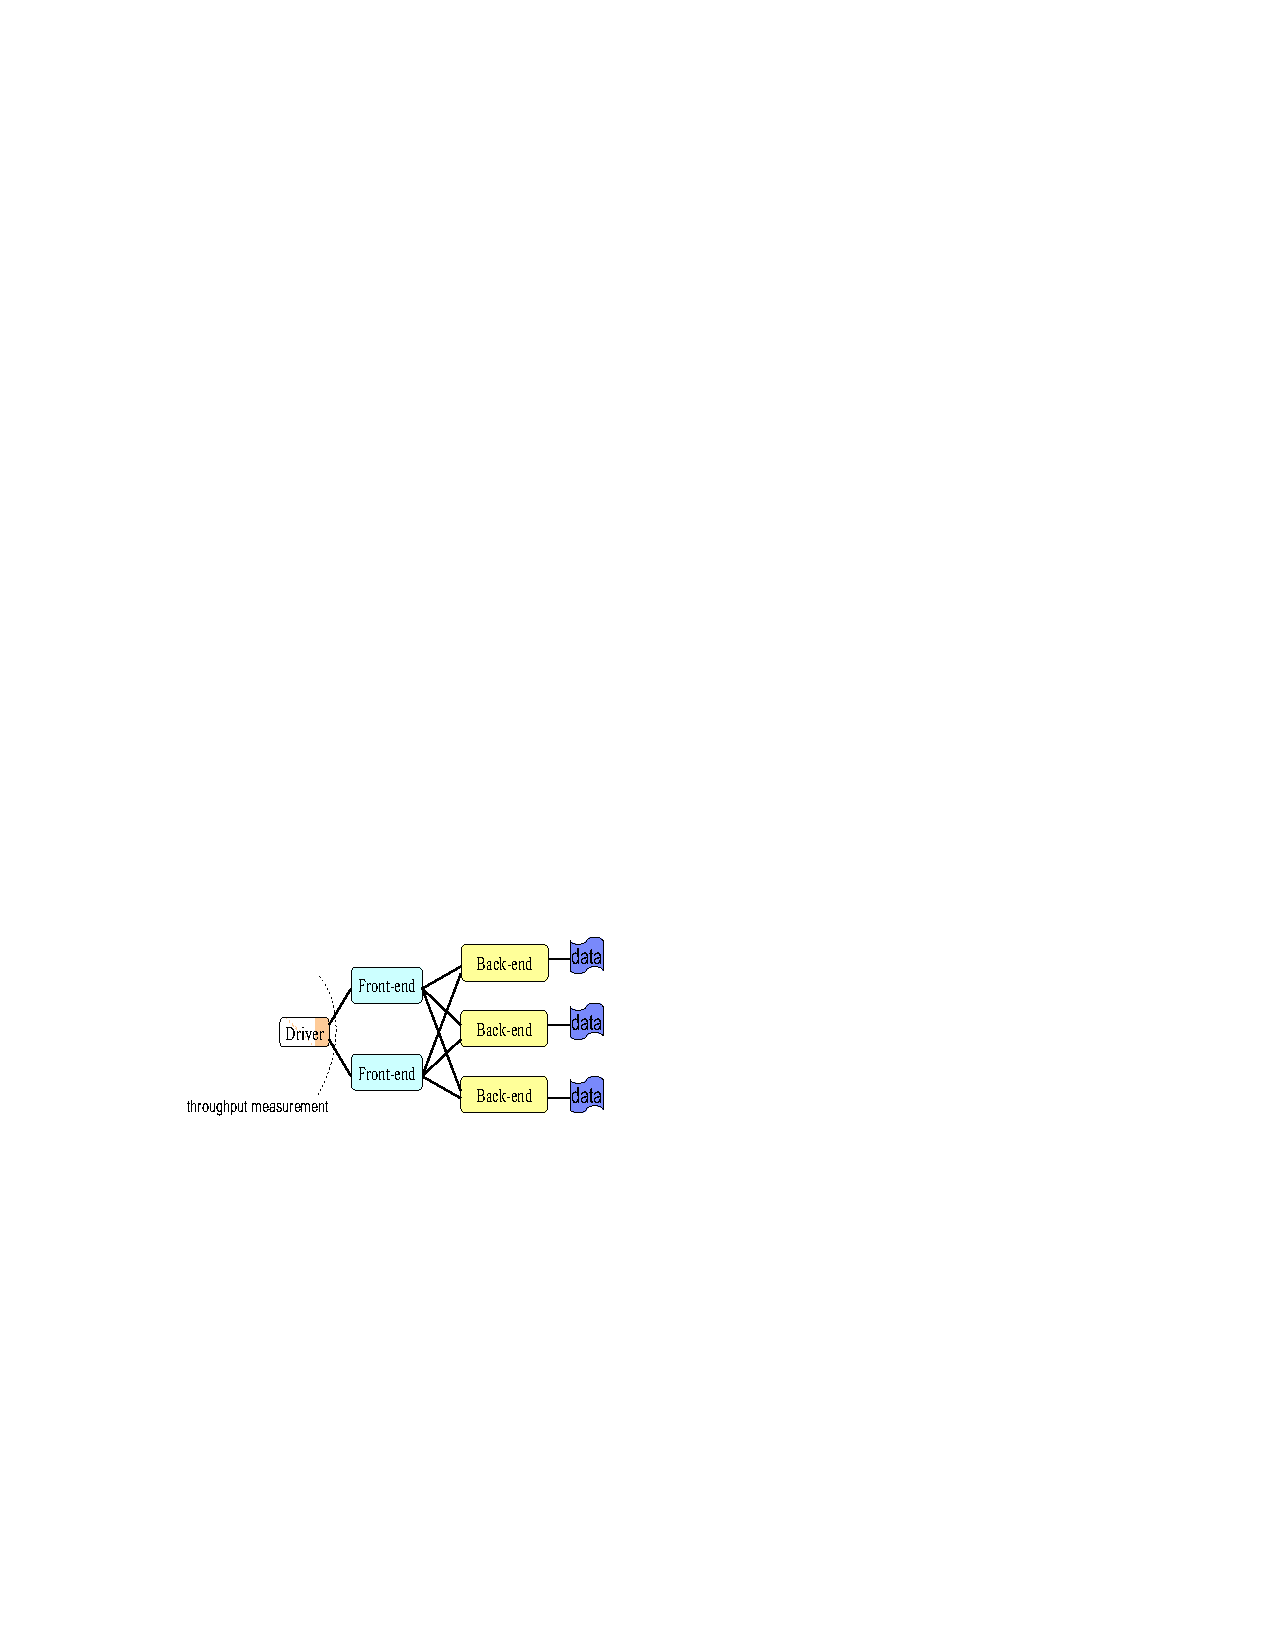
\includegraphics[width=0.5\textwidth]{Abbildungen/sharding}
    \caption[Horizonale Fragmentierung]{\footnotesize Abfragestruktur horizontal fragmentierter Systeme {\footnotemark} }
    \label{fig:sharding}
\end{figure}
\footnotetext{Quelle: \citep{Michael07}}

Der Nachteil einer derartigen Verteilung ist, dass Transaktionen um atomare Operationen zu gewährleisten erheblichen Zusatzaufwand nach sich ziehen. In Bereichen wo diese nicht notwendig sind, etwa bei der Verwaltung von Suchindexen, kann horizontale Fragmentierung allerdings zu signifikanten Leistungssteigerungen führen. \citep{Michael07}

\subsubsection{MapReduce basierte Algorithmen}

Liegen die Daten in einem verteilten System vor, muss auch die Verarbeitung über viele Systeme verteilt werden. Mit \textit{MapReduce} wird in \citep{mapred04} ein dafür geeignetes Programmier-Paradigma vorgestellt. 

 Die Eingabe- und Ausgabedaten der Verarbeitung bestehen aus einfach strukturierten Parameter-Wert Paaren (engl. Key-Value Pairs), welche in den drei festen Phasen \textit{Map}, \textit{Shuffle} und \textit{Reduce} verarbeitet werden. In der \textit{Map}-Phase wird jeder Datensatz einzeln und unabhängig von anderen durch die Anwendung verarbeitet. Die Unabhängigkeit ermöglicht es, diesen Schritt auf viele parallele Prozesse zu verteilen und die Verarbeitung sehr ``nah'' bei den Daten --- also über das gesamte verteilte System hinweg --- durchzuführen. Die Ergebnisse der Verarbeitung --- wiederum ein Parameter-Wert Paar --- werden in der darauffolgenden  \textit{Shuffle}-Phase entsprechend der Parameter sortiert. In der abschließenden  \textit{Reduce}-Phase werden alle zu einem Parameter gehörenden Werte gemeinsam verarbeitet. Die Verarbeitung der Gruppen erfolgt wieder unabhängig von anderen, so dass auch dieser Schritt auf viele parallele Prozesse und Rechenknoten verteilt werden kann. \citep{mapred04} \todo[color=green]{Ggf. MapRed. Beispiel einfügen.}

Trotz des sehr einfachen Verarbeitungsschemas ist es möglich, komplexe Algorithmen mit \textit{MapReduce} auszuführen. In \citep{mapred06} werden für zahlreiche Algorithmen des maschinellen Lernens die dafür notwendigen Umformungen beschrieben und analysiert. Grundlage der Umformungen ist das in \citep{Kearns98} beschriebene \textit{Statistical Query Model}. Dieses ermöglicht es, statistische Konzepte für Testdatensätze zu untersuchen und aus diesen darin vermutete statistische Verteilungen abzuleiten. Auf dieser Basis beschreibt \citep{mapred06} wie spezielle Algorithmen umgeformt werden können, um diese durch die Bildung von Teil-Approximationen und nachgelagerte Zusammenfassung in eine verteilbare \textit{MapReduce} Form zu überführen. Die so umgeformten Algorithmen skalieren nahezu linear mit der Anzahl der verfügbaren Rechenknoten bzw. Prozessorkernen. Dass diese Umformungen auch für die in Abschnitt \ref{sec:filtermethods}  beschriebenen Algorithmen des kollaborativen Lernens möglich sind, wird in \citep{jiang11} gezeigt. \citep{mapred06} \todo{BSP}

\subsubsection{Skalierung der Filtermodelle}

Die zuvor beschriebenen allgemeineren Methoden zur Verteilung und Verarbeitung großer Datenmengen sind im Zusammenhang mit Filtermodellen (vgl. Abschnitt \ref{sec:filtermethods}) vor allem im Bereich der Vorverarbeitung bzw. des Trainings relevant. 

Geht man davon aus, dass zur Verarbeitung eines einzelnen Bewertungseintrages 48 Byte im Speicher belegt werden, so stößt man bei ``üblichen'' 16 GB Hauptspeicher nach ca. 300 Millionen Einträgen an die Grenzen eines einzelnen Knotens. Auch wenn effizientere Speichernutzung --- etwa durch die Reduktion von Objektreferenzen --- den Speicherbedarf pro Eintrag auf 28 Byte senkt (vgl. \citep{mia}), ist es dennoch ratsam erheblich früher verteilte Algorithmen zu nutzen. Wie \citep{mapred06} und \cite{jiang11} zeigen, profitieren Systeme mit mehreren Prozessorkernen ebenfalls signifikant von der Parallelisierung durch \textit{MapReduce}.

Da die Laufzeit aller in Abschnitt \ref{sec:filtermethods} beschriebenen Modelle von der Anzahl der Nutzer und Elemente anhängig ist, machen es große Datenmengen zudem sehr schwer Empfehlungen ``online'' zu berechnen. Die Reduktion der verarbeiteten Informationen (zB. durch Cluster-Mechanismen) ist eine möglicher Ausweg. Da dadurch allerdings auch Informationen verloren gehen, sind die resultierenden Ergebnisse auch ungenauer. Einen möglichen Kompromiss zur Erzeugung von schnellen und präzisen Ergebnisse beschreibt \citep{linden03}. Alle rechenaufwendigen Verarbeitungsschritte, wie zum Beispiel die Berechnung von Element- oder Nutzerähnlichkeiten (vgl. Abschnitt \ref{sec:neighborhoods}), werden in eine Vorverarbeitungsphase verschoben und nur die eigentliche Generierung der Empfehlungen geschieht ``online''. Als Ergebnis der Vorverarbeitung erhält man entsprechend eine Matrix die Nutzer zu allen anderen Nutzern bzw. Elemente zu allen anderen Elementen korreliert. Der Rechenaufwand zur Generierung der Empfehlungen ist dann nur noch abhängig von der Anzahl der vom Nutzer gekauften bzw. bewerteten Elemente. Ein wichtiger Nachteil ist, dass neue Daten erst verspätet in das abgeleitete Filtermodell einfließen können, dies kann abhängig von der ``Stabilität'' der Datenbasis, zum Beispiel wenn Elemente nur kurze Zeit ``verfügbar'' sind (vgl. \citep{Cornelis20074906}), ein Ausschlussfaktor für Offline-Berechnungen sein. \citep{linden03}


%
% - Recommendation Datenmodelle die "schnell" sind
% - die meisten arbeiten mit "In-Memory" Datenmodellen (mit Optimierte Speicherung für die Ausführung)
%        - Wo sind die Grenzen (user,item anzahl ?)
%        - Lösungen: Precomputing similarities? 
%  - Lösungen: Cluster-based recommendation
%- Wann macht distributed recommendation sinn
%  - Ist Offline recommendation dafür ein Use-Case (Calculation recommendations and send via mail)?
%  - Das lernen der Datenmodelle muss auch skalieren
%- Hadopp etc...
%
%\citep{Vidal:2005:PDR:2137725.2137737}
%\citep{Toscher:2008:INA:1722149.1722153}
%http://techblog.netflix.com/2012/06/scalable-logging-and-tracking.html
%\subsubsection{Online- / Offline-Recommendation}
% BigTable http://labs.google.com/papers/bigtable-osdi06.pdf 
\subsection{Qualitätsmaße}\label{sec:measures}
%
%	\begin{itemize}
%	\item Successful session \citep{hb_18,Smyth05alive-user}
%	\item Precision /Recall /F1, \citep{rs}[Kap. 7]
%	\item User- und Itemcoverage \citep{rs}[S. 183]
%	\item Conversion / Click-through rates -> Joachim05 \\
%	Clickthrough ist als absolutes Maß eher problematisch da der Nutzer zum einen beeinflusst wird durch das Vertrauen in die Suchmaschine und durch die Qualität der sonst angebotenen Suchergebnisse. Bei einem Klick in einer Suchergebnisliste ist es deshalb sinnvoller die Relevanz abhängig von den nicht geklickten Elementen zu messen. (Joachim05)
%	\end{itemize}
%
%Zusammenfassung aus Cacheda11, Cremonesi10, Joachim05 und Herlocker04

Im folgenden Abschnitt werden verschiedene Wege zur Bewertungen von Empfehlungsdiensten beschrieben. Sie dienen zum qualitativen Vergleich von Filtermodellen und als Kontrollwerkzeug vor und während der Inbetriebnahme des Dienstes.

\subsubsection{Mittlere Abweichung} \label{sec:qa_rmse}

Eine naheliegende Methode zum Vergleich von Filtermodellen ist es, deren Fehlerquote in Bezug zu vorliegenden historischen Nutzerdaten zu bestimmen, bzw. zu messen wie stark die ermittelten Werte von den tatsächlichen abweichen. Hierfür wird oft der \textit{mittlere absolute Fehler} (engl. \acf{MAE}) oder die \textit{Wurzel aus dem mittleren quadratischen Fehler} (engl. \acf{RMSE}) genutzt.

Auf der Basis einer Testmenge $\mathcal{T}$ wird für alle darin befindlichen Nutzer-Element-Paare $(u,i)$ der berechnete Ratingwert $\hat{r}_{ui}$ mit dem tatsächlichen $r_{ui}$ vergleichen.

Die beiden Fehlermaße werden dann wie folgt gebildet:
\begin{align}
MAE & = \frac{1}{|\mathcal{T}|} \sum_{(u,i) \in \mathcal{T}}{|\hat{r}_{ui}-r_{ui}|} \label{form:mae} \\
RMSE & = \sqrt{\frac{1}{|\mathcal{T}|} \sum_{(u,i) \in \mathcal{T}}{(\hat{r}_{ui}-r_{ui})^2}} \label{form:rmse}
\end{align}

Der Unterschied zwischen den Methoden liegt in der Bewertung großer Fehler. Wie in Tabelle \ref{tab:mae-rmse} gezeigt wird, kann dies durchaus ausschlaggebend sein. Im Beispiel werden zwei Modelle $\hat{r}_{(i)}$ miteinander verglichen. Das Modell $\hat{r}_{(1)}$ wird vom \acs{MAE} bevorzugt, da der einzige Fehler durch die drei richtigen Werte stärker ausgeglichen wird. Beim Vergleich mit dem \acs{RMSE} wird Modell $\hat{r}_{(2)}$ bevorzugt, da die vier kleinen Fehler in $\hat{r}_{(2)}$ weniger ins Gewicht fallen als der größere Fehler in $\hat{r}_{(1)}$. \citep{hb_08} \\ \\
\begin{SCtable}[][h]
  \centering
  \begin{tabular}{ | r | p{1cm} | p{1cm} | p{1cm} | }
    \hline
    & $r$ & $\hat{r}_{(1)}$ & $\hat{r}_{(2)}$ \\ \hline
    Item1 & 3 & 3 & \underline{2} \\
    Item2 & 4 & \underline{1} & \underline{2} \\
    Item3 & 2 & 2 & \underline{3} \\
    Item4 & 3 & 3 & \underline{2} \\ \hline \hline
    MAE & & \textbf{0.75} & 1.25 \\
    RMSE & & 1.5 & \textbf{1.32} \\
    \hline
  \end{tabular}
  \caption[Beispielrechnung zum Vergleich von \acs{MAE} und \acs{RMSE}]{\footnotesize Beispielrechnung zum Vergleich von \acs{MAE} und \acs{RMSE} - gegenübergestellt sind tatsächliche Bewertungen $r$ und von zwei verschiedenen Quellen erzeugte angenommene Bewertungen $\hat{r}_{(1)}$ und $\hat{r}_{(2)}$. Abweichende Bewertungen sind unterstrichen. { \scriptsize  (eigene Darstellung) }}
  \label{tab:mae-rmse}
\end{SCtable}

\subsubsection{Trefferquote und Genauigkeit}\label{sec:precision}

Wird eine Liste von Empfehlungen erzeugt, kann neben der möglichen Bewertung und deren Genauigkeit auch gemessen werden, ob und wieviele der Empfehlungen korrekt waren. Bei der Evaluierung mit historischen Daten werden hierzu aus einem Nutzerprofil eine Reihe von Elementen entfernt und für das abgeleitete Profil eine Liste von Empfehlungen erzeugt.

Durch den Vergleich der entfernten Elemente mit den Empfehlungen können dann \textit{Genauigkeit} $P$ (engl. Precision) und \textit{Trefferquote} $R$ (engl. Recall) wie folgt gemessen werden:
\begin{align}
P_u & = \frac{|hits_u|}{| recset_u | } \label{form:precision} \\
R_u & = \frac{|hits_u|}{ | testset_u | } \label{form:recall}
\end{align}

Die Anzahl der korrekt empfohlenen Elemente $hits_u$ wird zur Anzahl aller empfohlenen Elemente $recset_u$ bzw. zur Anzahl der möglichen richtigen Empfehlungen $testset_u$ ins Verhältnis gesetzt. Die Verbesserung beider Werte steht dabei oft im Widerspruch zueinander. So kann durch die Vergrößerung der Anzahl von empfohlenen Elementen auch die Wahrscheinlichkeit von Treffern und damit die Trefferquote gesteigert werden. Allerdings hätte die insgesamt gestiegene Zahl von Empfehlungen auch einen negativen Einfluss auf die Genauigkeit. Zur Kombination beider Werte kann die $F_1$ Metrik genutzt werden. Sie gewichtet beide Werte mit einer Neigung zum schlechteren.
\begin{align}
F_1 & = \frac{2 * P * R}{P+R} \label{form:f1}
\end{align}

Die ebenfalls mögliche Bestimmung der Ausfallquote (engl. Fallout), also der Anzahl der nicht korrekt empfohlenen Elemente im Verhältnis zur Menge aller Elemente, wird seltener zur Bewertung von Ergebnissen herangezogen. \citep{hb_08,rs}

\subsubsection{Empirische Messung}\label{sec:measure_c}

Ergänzend zur Messung der Approximationsgüte des erzeugten Modells muss bei einem praktischen Einsatz auch der tatsächliche Erfolg der eingesetzten Methode gemessen werden. Dafür bieten sich die aus dem Marketing stammenden \textit{Klickraten} und \textit{Conversion-Raten} Messung an, des weiteren kann in Verbindung mit Suchindexen auch die Bestimmung der \textit{Successful Session} Quote genutzt werden.

\paragraph{Klickrate} Beschreibt die Anzahl der Klicks auf ein Element, zum Beispiel einen Werbebanner, im Verhältnis zur Häufigkeit mit der es angezeigt wurde. 

\paragraph{Conversion-Rate} Mit der Conversion-Rate wird bestimmt welcher Anteil der Besucher ein bestimmtes Ziel, die sog. \textit{Conversion}, erreicht haben. Mögliche Ziele sind zum Beispiel erfolgreiche Kaufabschlüsse oder Kontaktaufnahmen der Kunden. Die Ziele werden abhängig vom Kontext so gewählt, dass diese aktiv zur Wertschöpfung beitragen. Die Berechnung der Conversion-Rate entspricht gem. Formel (\ref{form:cr}) dem Verhältnis der gemessenen Anzahl an Conversions $conv$ und der Anzahl der Besucher $visitors$ die im gegebenen Zeitraum eine oder mehrere Seiten aufgerufen haben. Maschinelle Seitenzugriffe, zum Beispiel durch Suchmaschinen-Spider, fließen nicht in die Messung der Nutzerzahlen ein. Ebenso werden wiederholte Conversions des gleichen Besuchers nicht mehrfach gezählt. \citep{krueger2011conversion}
\begin{align}
CR & = \frac{|conv|}{|visitors| } * 100 \label{form:cr}
\end{align}

\paragraph{Successful Session}\label{sec:successfulsession} Da die Nutzeroberfläche von Suchmaschinen in der Regel kein explizites Feedback vom Nutzer zur Qualität der gefundenen Ergebnisse  zulässt, muss die Relevanz einer Ergebnisliste über implizite Verfahren gemessen werden. In \citep{smyth05a} wird die Methode der \textit{Successful Session} für diesen Zweck beschrieben. Die Ergebnisliste einer Suche wird demnach immer dann als relevant bewertet, wenn der Nutzer mindestens eines der Ergebnisse ausgewählt hat. Wird keines gewählt, wird die Liste entsprechend als irrelevant bewertet. Eine weitere Abstufung bzw. Steigerung der Relevanz, zum Beispiel bei wiederholter Ergebniswahl, wird nicht getroffen. \citep{smyth05a} % \todo[color=green]{HB Kap. 10.4.2 dazu?}
%\subsubsection{Normalisierter DCG}
%\subsubsection{A/B Testing}
